本章节首先将会介绍与本文相关的研究工作,包括对于API文档的研究,对于Stack Overflow网站的研究,以及前人所做的在Stack Overflow上进行API知识抽取的研究。其次,本章节还会介绍本文使用到的一些方法与工具,如使用的信息抽取技术和自然语言处理技术等。

\section{API文档与Stack Overflow相关研究}
Robillard和Deline等人\cite{DBLP:journals/ese/RobillardD11}针对开发人员在学习API时遇到的困难进行了一系列经验研究。该研究设计了一系列对专业软件开发人员的调查和访谈,包括:

\begin{enumerate}
    \item 一项探索性的问卷调查,用于确定学习障碍的类别。
    \item 一组定性访谈调查,用于收集在工作中遇到的API学习障碍的具体场景。
    \item 一项后续问卷调查,用于确认该研究的结论并收集更多可能影响API学习障碍的额外因素。
\end{enumerate}

该研究在微软公司中展开,收集了440名专业软件开发者的调查结果。通过对调查结果进行分析,研究者发现开发人员在学习新API时面对的最大障碍来自于API文档的不足。而API文档的缺失体现在多个方面,如缺失与API的设计和原理相关的信息,缺少与使用场景相关的信息,缺少对API错误的处理指导以及缺少示例代码等等。

Mamykina等人\cite{DBLP:conf/chi/MamykinaMMHH11}对Stack Overflow进行了一系列的分析,她们通过将统计数据分析和用户访谈两种方法相结合\cite{DBLP:conf/chi/NamAA09},分析了Stack Overflow在软件工程领域取得成功的原因。该工作首先对整个Stack Overflow语料库进行分析,分别调查了回答时间、用户类型、不同问题类型的适用以及Stack Overflow这样的问答网站模型对其他领域是否可能存在拓展性,然后对网站的用户以及网站设计者进行了定性访谈研究。在软件工程领域,Stack Overflow取得了巨大的成功,网站上的问题回答率超过了90\%,远高于其他类似的问答网站,平均每个问题的回答耗时仅有11分钟。在用户访谈中,有许多用户认为Stack Overflow已经取代了搜索引擎,成为了他们解决编程问题的主要手段,同时还有一些用户认为自己在Stack Overflow网站上的高质量回答能为自己的简历增色不少。最后,Mamykina等人将Stack Overflow在软件工程领域的成功总结为精心设计的社区声誉系统,严格的社区准则,以及设计团队在自己设计的社区中积极地参与。

Treude等人\cite{DBLP:conf/icse/TreudeBS11}对Stack Overflow上提出的问题进行分类,并对不同类型问题的回答情况进行分析。该研究首先从Stack Overflow提供的API接口中获得了2010年11月1日至11月15日期间被提出的问题,并对这些问题进行定性分析和定量分析。通过对这些问题带有的标签以及问题标题与问题正文中出现的关键字进行分析,Treude等人将Stack Overflow上问题的标题分成10个类别,如表\ref{表2-1}所示。其中,出现频率最高的问题类型是how-to类型的问题。

\begin{table}[h]
    \centering
    \caption{Stack Overflow帖子标题分类\cite{DBLP:conf/icse/TreudeBS11}}
    \label{表2-1}
    \begin{tabular}{ll}
    \hline
    类别             & 具体描述                \\ \hline
    how-to         & 与寻求具体实现的指导相关的问题     \\
    discrepancy    & 作者想要得到解释的一些意外情况     \\
    environment    & 开发期间或部署后有关环境的问题     \\ 
    error          & 包含特定错误消息的问题         \\
    decision help  & 与意见征求相关的问题          \\
    conceptual     & 抽象且没有具体用例的问题        \\
    review         & 隐含或明确要求代码审查的问题      \\
    non-functional & 关于性能或内存使用等非功能性需求的问题 \\
    novice         & 明确指出提问者是一个新手        \\
    noise          & 与编程无关的问题          \\ \hline 
    \end{tabular}
\end{table}

在Treude等人的研究基础之上,Abdalkareem等人\cite{DBLP:journals/software/AbdalkareemSR17}针对开发人员如何使用Stack Overflow帮助自己完成编程任务继续进行了研究。该工作首先从GHTorrent数据集\cite{DBLP:conf/msr/Gousios13}中获取当前最流行的编程语言编写的Github项目,并从中筛选出较为活跃且成熟的项目。通过筛选设定条件为至少有100个pull request、至少有3个及以上开发人员以及过去的一年内至少有100次代码提交,Treude等人从数据集中找出那些符合要求的Github项目,再从这些项目的代码提交中找出那些提交日志中包含有Stack Overflow字样的,最后得到1780个符合条件的代码提交。通过对这些代码提交及其相关的Stack Overflow帖子进行人工统计,该工作将开发人员在Stack Overflow上寻求帮助的帖子分成了14个类别,如表\ref{表2-2}所示。

% Please add the following required packages to your document preamble:
% \usepackage{multirow}
\begin{table}[h]
    \centering
    \caption{Stack Overflow帖子知识需求分类\cite{DBLP:journals/software/AbdalkareemSR17}}
    \label{表2-2}
    \begin{tabular}{|c|c|c|}
    \hline
    主题                         & 副题          & 百分比   \\ \hline
    \multirow{9}{*}{运用知识}      & 编程语言        & 22.07 \\ \cline{2-3} 
                               & API使用       & 21    \\ \cline{2-3} 
                               & 配置管理        & 7.21  \\ \cline{2-3} 
                               & Web框架       & 6.51  \\ \cline{2-3} 
                               & Web浏览器      & 4.31  \\ \cline{2-3} 
                               & 开发工具        & 4.17  \\ \cline{2-3} 
                               & 实现问题        & 3.89  \\ \cline{2-3} 
                               & 数据库技术       & 2.83  \\ \cline{2-3} 
                               & 操作系统        & 2.4   \\ \hline
    \multicolumn{2}{|c|}{文档错误}               & 13.08 \\ \hline
    \multicolumn{2}{|c|}{Stack Overflow网站相关} & 3.18  \\ \hline
    \multicolumn{2}{|c|}{特性或系统改进}            & 1.77  \\ \hline
    \multicolumn{2}{|c|}{代码重用}               & 1.7   \\ \hline
    \multicolumn{2}{|c|}{其他}                 & 5.87  \\ \hline
    \end{tabular}
    \end{table}

该工作的统计数据表明,开发人员主要使用Stack Overflow来获取知识,常见的知识需求有编程语言特性、API使用、配置管理等,这部分Stack Overflow帖子占了数据集中的61.1\%。其次,开发人员还会使用Stack Overflow来记录自己在软件开发中遇到的错误,以及对于错误的解决方案等。这一部分类型的帖子在数据集中占有14.85\%。

从Abdalkareem等人的研究中我们不难得出结论,Stack Overflow的帖子中包含有许多有益于开发人员进行软件开发的知识,特别是与API相关的知识,这是本文选择Stack Overflow作为API知识抽取的语料库的原因。而通过Robillard等人的研究,我们可以得知现有的API文档无法满足程序员学习一个新API的需求。因此,许多开发者转而使用Stack Overflow作为学习新API知识的途径\cite{DBLP:conf/chi/MamykinaMMHH11}。在以上研究背景下,Stack Overflow具有作为API文档补充的巨大潜力,这也是所有基于Stack Overflow网站的API知识抽取研究工作提出的基础。

\section{API知识抽取相关研究}
为了从Stack Overflow网站上抽取出API知识并对API文档进行补充,国内外学者进行了许多研究工作。有部分学者使用了基于规则的抽取方式。Liu等人\cite{DBLP:conf/internetware/Liu0JMYZ18}采用了基于正则表达式和模式匹配的方法从多种属性的角度对Stack Overflow帖子中的知识进行分类,最后将帖子的知识分类结果用于设计一个Stack Overflow帖子的检索算法。Treude等人\cite{DBLP:conf/icse/TreudeBS11}的工作也基于规则匹配,他们设计了一些正则表达式来对Stack Overflow中的帖子标题和正文进行匹配,并对匹配得到的Stack Overflow帖子进行分类。这些工作有的是以较粗粒度的帖子作为对象的,也有的是以较为细粒度的句子级文本作为操作对象的。

此外,还有许多学者采用了基于机器学习的抽取方式。Treude等人\cite{DBLP:conf/icse/TreudeR16}在之前工作的基础上,提出了一种称为SISE的API知识抽取方法。如表\ref{表2-3}所示,SISE从了Stack Overflow帖子抽取出大量信息作为句子特征,包括句子文本本身,句子的语言模式,句子的归属问题,归属回答,帖子的作者,句子中的词性标签以及该句子与相应API文档的句子相似度等,并用这些句子特征训练了一个分类模型,用于从Stack Overflow帖子中抽取出带有API观点的句子。该工作的研究者人工标注了1574个来自Stack Overflow中的句子作为开发集,并通过实验证明了SISE在开发集上表现良好,能够达到0.64的准确率和0.7的覆盖率。

\begin{table}[h]
    \centering
    \caption{SISE方法中的句子特征\cite{DBLP:conf/icse/TreudeR16}}
    \label{表2-3}
    \begin{tabular}{ll}
        \hline
        \# & 特征                            \\ \hline
        1  & 句子与API文档中最相似句子之间的余弦相似度        \\
        2  & 句子与API文档中所有句子之间的平均余弦相似度       \\
        3  & 问题的用户接受率                      \\
        4  & 回答的得分                         \\
        5  & 回答的年龄                         \\
        6  & 回答耗时                          \\
        7  & 问题得分                          \\
        8  & 问题收藏数                         \\
        9  & 提问者的声誉                        \\
        10 & 问题的浏览次数                       \\
        11 & 句子中放在动词前的第三人称单数现在进行时形式的名词数量   \\
        12 & 问题的年龄                         \\
        13 & 句子是否以放在动词前的第三人称单数现在进行时形式的名词开头 \\
        14 & 句子包含的词语个数                     \\
        15 & 句子中API提及出现的位置                 \\
        16 & 句子中API提及出现的次数                 \\
        17 & 回答的得分                         \\
        18 & 回答的长度                         \\
        19 & 句子中名词的数量                      \\
        20 & 句子是否以名词开头                     \\
        21 & 句子中代码片段的字符数                   \\
        22 & 句子中单词“be”的出现次数                \\ \hline
    \end{tabular}
\end{table}

Uddin等人\cite{DBLP:journals/tse/UddinK21}针对Stack Overflow上讨论API的句子进一步拓展了前人关于软件工程领域情感分析方面的研究。在之前的研究中,有许多学者针对软件工程领域的文本情感分析进行了许多工作,如对Github上的评论进行情感分析\cite{DBLP:conf/kbse/UddinK17}\cite{DBLP:conf/msr/PleteaVS14}\cite{DBLP:conf/msr/GuzmanAL14}\cite{DBLP:conf/sigsoft/GuzmanB13},以及对传统的情感分析工具在软件工程领域的表现进行了实验对比\cite{DBLP:conf/icsm/JongelingDS15}。由于传统的情感分析工具在软件工程领域表现不佳,Uddin等人基于Hu和Liu等人\cite{DBLP:conf/kdd/HuL04}提出的主导情绪取向算法和Thelwall等人\cite{DBLP:journals/jasis/ThelwallBPCK10}实现的情感分析工具SentiStrength进行了改进,实现了更贴近软件工程领域需求的情感分析算法OpinerDSOSenti。同时,他们还设计了一系列调查,用于了解开发人员更喜欢在论坛上讨论关于API的哪些方面,并通过分析来自178名专业软件开发人员的回答将关于API的意见分成了11类,如表\ref{表2-4}所示。最后,Uddin等人使用OpinerDSOSenti算法在随机采样得到的1338个Stack Overflow帖子中对所有句子进行情感分析,并将抽取得到的带有情感倾向的句子分类到提出的11中类别中。该工作的抽取结果与人工标注的结果对比表明,OpinerDSOSenti在抽取带有情感倾向的句子方面准确率较高,达到了0.778,而在分类准确率上表现较为一般,仅有0.502的正确率。较低的分类准确率可能是由于作者设计的知识分类类型较多,模型不能很好地区分不同类型知识之间的特征。

\begin{table}[h]
    \centering
    \caption{Opiner工具对API意见的分类\cite{DBLP:journals/tse/UddinK21}}
    \label{表2-4}
    \begin{tabular}{|l|l|}
        \hline
        类别        & 定义                                                                      \\ \hline
        性能        & 与一个API的性能相关的观点                                                          \\ \hline
        可用性       & 一个API是否是好用的                                                             \\ \hline
        安全        & \begin{tabular}[c]{@{}l@{}}与安全原则、安全漏洞的影响以及对API最佳安全实现\\ 的观点\end{tabular} \\ \hline
        文档        & 该API在各种开发资源中是如何被记录的                                                     \\ \hline
        兼容性       & 该API在一个给定的框架中是如何工作的                                                     \\ \hline
        可移植性      & 该API是否能在不同的操作系统下工作                                                      \\ \hline
        社区        & 使用和开发该API的开发者是否能快速响应                                                    \\ \hline
        合法性       & 关于一个API的许可问题的观点                                                         \\ \hline
        漏洞        & \begin{tabular}[c]{@{}l@{}}关于该API的某个特定漏洞的存在、扩散以及修复的\\ 意见\end{tabular}   \\ \hline
        其他通用API特性 & 其他关于该API的特性或用法的意见                                                       \\ \hline
        情绪表达      & 只有情绪表达,而不涉及具体方面的观点                                                      \\ \hline
        \end{tabular}
        \end{table}

\section{基于自举(Bootstrapping)思想的信息抽取技术}
从知识图谱这一学科建立以来,知识抽取就一直是该领域研究的一个重要方向。在机器学习技术非常成熟的今天,许多学者更倾向于结合最新的深度学习技术来取得更好的知识抽取效果。然而,在工业界,基于自举思想的自举抽取法作为一种老而弥坚的知识抽取方法仍然能在较低的技术门槛下取得非常好的效果。该方法最早由Brin在1998年提出\cite{DBLP:conf/webdb/Brin98},这是一种被命名为DIPRE(Dual Iterative Pattern Expansion)的半监督的结构化关系抽取方法,能够通过在非常少的实例中学习种子模板,然后在大量非结构化文本中使用这些种子模板抽取出新的实例,同时在抽取出的新实例中学习得到新的模板,并继续使用这些新的模板抽取实例。DIPRE方法的工作流程如图2-1所示。

\begin{figure}[htb]
    \centering
    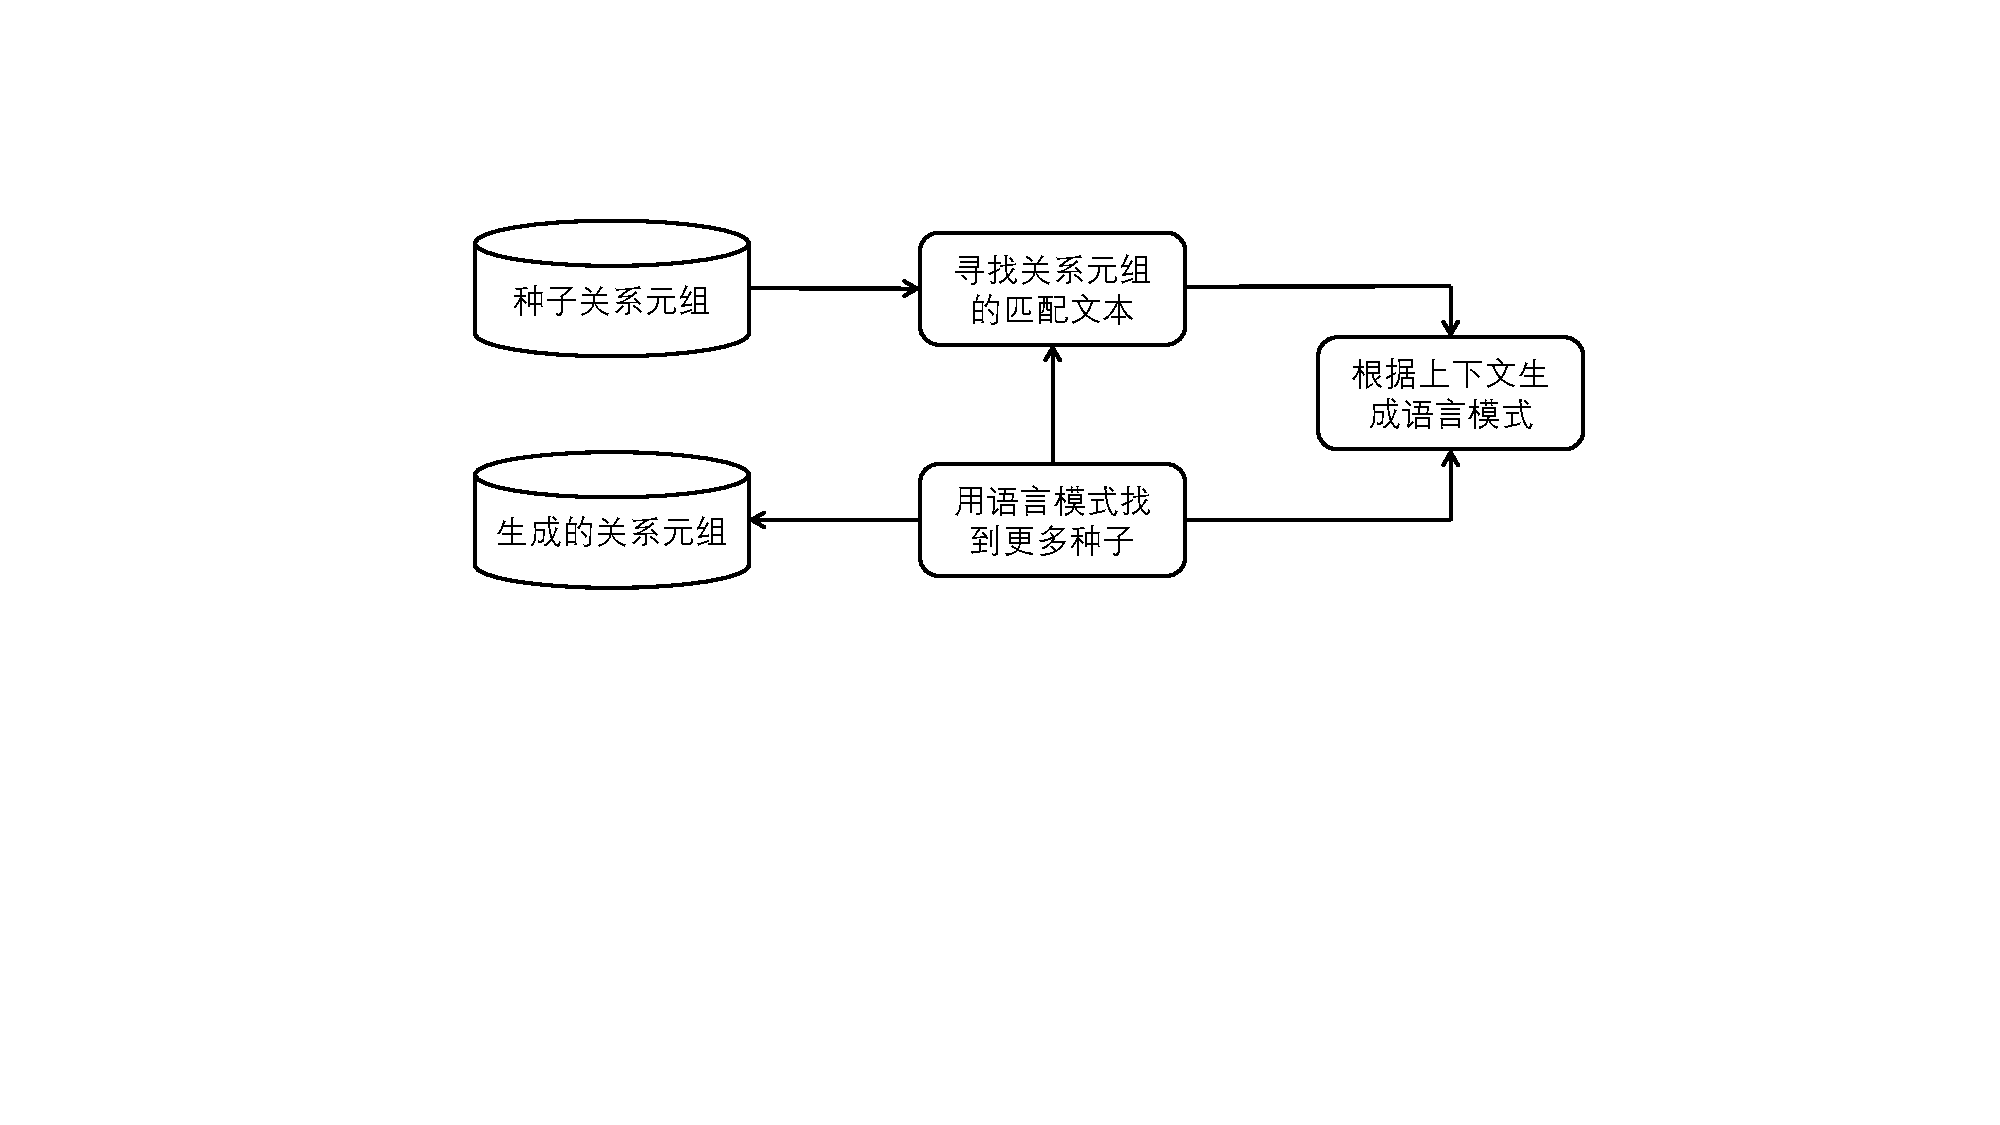
\includegraphics[width=\textwidth]{image/DIPRE.pdf}
    \caption{DIPRE方法工作流程\cite{DBLP:conf/webdb/Brin98}} 
    \label{fig:fig1} 
\end{figure}

Agichtein\cite{DBLP:conf/sigmod/AgichteinGV01}在Brin的基础之上对方法进行了改进,设计实现了Snowball信息抽取系统。与DIPRE相比,由Snowball抽取出来的模板包含了来自种子的命名实体标签,并且设计了一种用于在抽取的过程中评估每次迭代生成的模板和种子的策略,在迭代抽取信息的过程中只保留那些被认为是可靠的种子和模板。通过这些优化设计,Snowball系统取得了比DIPRE更好的效果,在Agichtein设计的对比实验中,Snowball系统和DIPRE系统得到了相近的精确率,但Snowball的召回率更高。

在这之后,还有许多学者基于DIPRE方法继续进行优化,如Carlson等人\cite{DBLP:conf/aaai/CarlsonBKSHM10}设计了NELL(Never-Endding Language Learner)知识抽取系统,只需提供一个种子模式,就能在大规模的Web文本上迭代地抽取知识,并通过对抽取出来的文本知识打分来提高抽取的准确率。

本文也是基于自举思想实现的知识抽取方法,针对软件工程领域设计了特定的知识概念模型,并针对API知识这一抽取目标设计了合理的知识抽取方法。

\section{自然语言处理工具}
本小节将会介绍本文使用到的与自然语言处理的相关工具,包括自然语言解析工具spaCy,以及它提供的数个模块,还有Facebook公司提出的文本分类算法fastText,以及该算法的封装库。
\subsection{spaCy及其原理}
spaCy\footnote{https://spacy.io/}是一个用于自然语言处理的Python开源模块,可以用于构建处理和理解大量文本的程序。得益于在许多相关模块使用Cython(一种Python的C语言拓展,旨在让Python程序的性能够接近C语言程序)进行优化,spaCy的性能非常强大,与科研工作常用的Python自然语言处理库NLTK相比,它的解析速度更快,且为CPU进行了针对性优化,这让spaCy在没有GPU的环境下也能很好地工作。

spaCy提供了非常简便的调用方式来对自然语言文本进行处理,包括文本清洗、分词、分句、命名实体识别、词干化、词性标注和依赖解析功能等,这些都基于已经训练好的机器学习和深度学习模型(如BERT等)实现。spaCy的可拓展性非常强,用户可以根据自己的需要对整个文本处理流程进行定制,增加、修改自己所需要使用的管道组件,并移除自己所没有使用到的文本处理模块。spaCy的高可拓展性进一步提高了它的性能。

spaCy中的Tokenizer模块用于支持分词、分句功能,它由前缀模式、中缀模式、后缀模式和特殊规则组成。在文本处理的过程中,spaCy先将文本进行简单的空格分词,Tokenizer再从左向右依次处理词语,检查词语是否匹配特殊规则、或者是前中后缀中的一种,再根据这些模式进行分词。本文中对spaCy的优化主要是对Tokenizer模块的修改,让spaCy的分句、分词更加契合Stack Overflow网站上的讨论文本,如适应API提及句子的分句、适应对特殊符号的分词等,提高数据的整体质量。

spaCy还提供了Matcher模块,允许用户制定规则进行文本匹配,匹配的规则可以是基于文本,基于词性标签,或者基于词法属性。与文本匹配常用的正则表达式相比,spaCy的Matcher模块不仅能找到符合规则的文本,还能对文本中的单词进行访问,获得其词性等属性,或者在单词级别对文本进行修改。本文使用到了Matcher模块用于从一个描述了API知识的句子中抽取出代表该种API知识表达方式的语言模式,并用这些模式在语料库中寻找相似的句子。

除了Matcher模块之外,spaCy还为用户提供了PhraseMatcher模块。PhraseMatcher模块提供了同时检索多个词语的方法。通过将需要检索的词汇表添加到一个PhraseMatcher中,就能实现快速判断一个句子是否包含词汇表中的所有单词。这种判断方式比常规的字符串匹配更为高效,故本文使用了这一模块作为从语料库中匹配API知识的方式,从而提高方法流程的整体效率。

\subsection{fastText}
fastText\footnote{https://fasttext.cc/}是由Facebook公司开源的一个用于文本分类的Python开源模块,通常用于带监督的文本分类问题。fastText算法在学术上并没有非常显著的创新,但它结合了在自然语言处理与机器学习领域中已有的优秀算法,这让它在拥有与基于深度学习算法的文本分类器不相上下的高精度的同时还具有更快的模型训练速度以及预测速度。

在机器学习技术已经发展得非常成熟的今天,基于神经网络的文本分类技术在实践中表现优异,但它们在训练和测试时往往较慢,这一特点限制了基于神经网络的文本分类技术在大型文本数据集上的运用。同时,过去的线性文本分类技术虽然已提出多年,但在选择合适的句子特征作为输入时,它的表现并不比基于神经网络的分类器差。

因此,Joulin等人提出了fastText方法\cite{DBLP:conf/eacl/GraveMJB17},将早期的线性文本分类技术进行优化,大大提高了它在大型文本数据集上运行的效率。fastText算法的模型结构如图\ref{图2-1}所示。fastText算法使用了词袋特征以及n-gram特征来表征一个句子,通过线性变换来将这些句子特征映射到模型架构的中间层中,再使用一个基于哈夫曼编码的层次softmax分类器将句子分类到特定的标签中。由于线性文本分类器在特征和类别之间不共享参数,这可能会影响到它在大型文本数据集上的泛化表现。为了解决这一问题,Joulin等人将线性分类器分解为低秩矩阵。

\begin{figure}[htb]
    \centering
    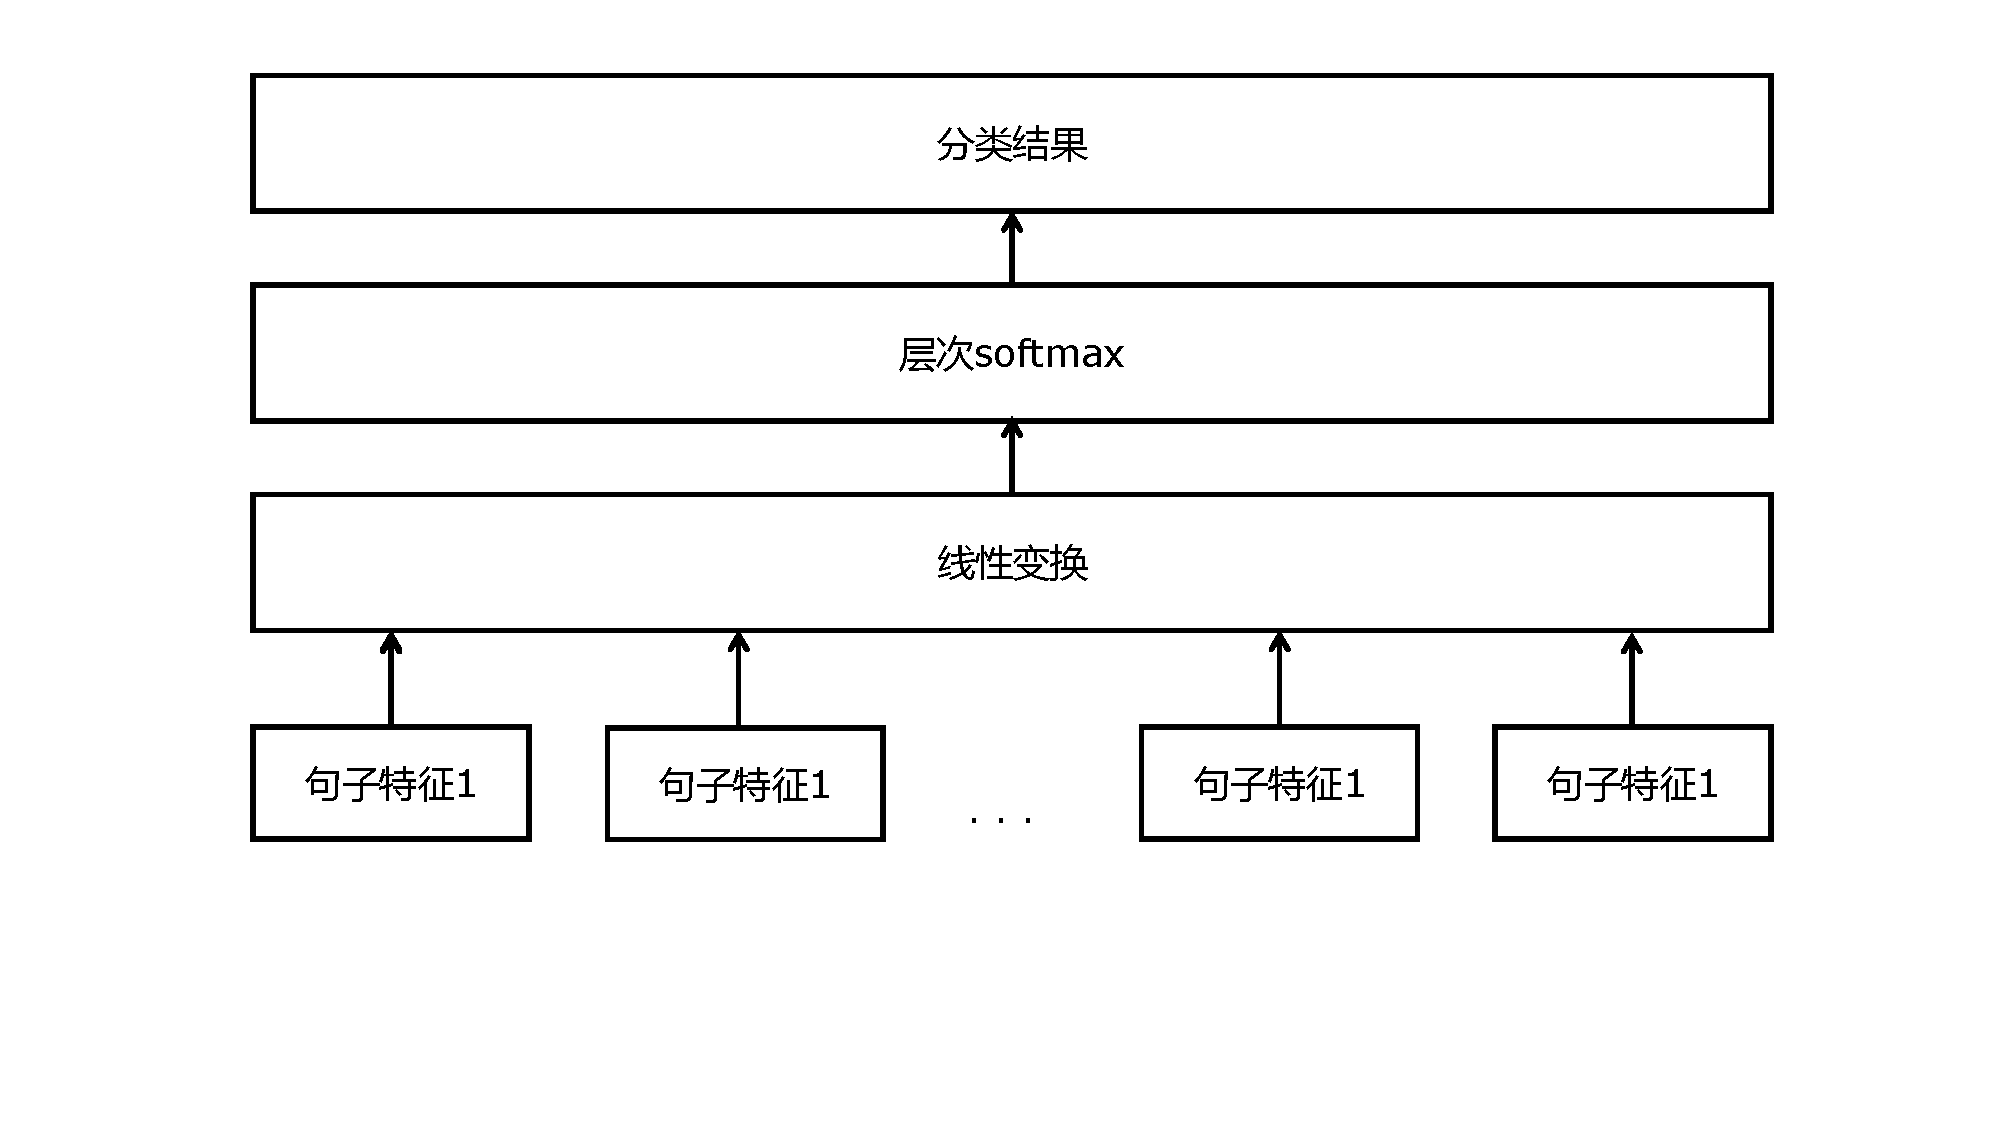
\includegraphics[width=\textwidth]{image/fast-text.pdf}
    \caption{fastText模型结构\cite{DBLP:conf/eacl/GraveMJB17}} 
    \label{图2-1} 
\end{figure}

当分类的类别过多时,标准的归一化softmax效率较低,时间复杂度是O(kh),其中k是类别的数量,h是文本表示的维度。为了提高速度,Joulin等人通过使用基于哈夫曼编码树的分层softmax,使得计算一个句子所属类别的时间复杂度降低到O(hlog2(k))。这让fastText在计算一个句子分类到某个标签的概率的速度大大地提高了。

Facebook公司开源的Python第三方库 fastText 提供了fastText算法直观易用的调用方式,让用户不需要预训练词向量,只需提供预标注的训练数据就可以在极短的时间内训练出一个高精度的文本分类器。与传统的基于神经网络的文本分类器相比,fastText的训练速度要快上若干个数量级。在标准的多核CPU上,fastText能够在10分钟之内训练10亿个词级别的语料库的词向量,并且能够在1分钟内将具有30万种类别的50多万条句子完成分类。

本文使用了fastText库,预标注并训练出一个文本分类器用于识别出Stack Overflow帖子中的API描述性知识句子,通过这种方式来生成一个高质量的语料库,保证了本方法抽取出来的知识的质量。

\section{本章小结}
本章主要介绍了与API文档,Stack Overflow和API知识抽取技术的相关研究,以及本文所使用到的相关技术。本章首先介绍了与API文档和Stack Overflow网站相关的研究,说明了对于软件开发人员来说API文档并不足以满足日常开发需求,而Stack Overflow网站上包含有大量与API相关的众包知识能够作为API文档的补充。之后介绍了其他学者基于Stack Overflow网站进行的API知识抽取工作,包括基于规则和基于机器学习的方法。然后介绍了基于自举思想的信息抽取技术,以及它的衍生工作。最后,本章还介绍了本方法中使用到的一些工具,包括自然语言处理工具spaCy和文本分类器fastText。
